%!TEX root = *.tex
%%%%%%%%%%%%%%%%%%
% カウンタのリセット
\setcounter{figure}{0}
% 問題文
{
\begin{wrapfigure}{r}{12zw}
  \vspace{-\intextsep}
  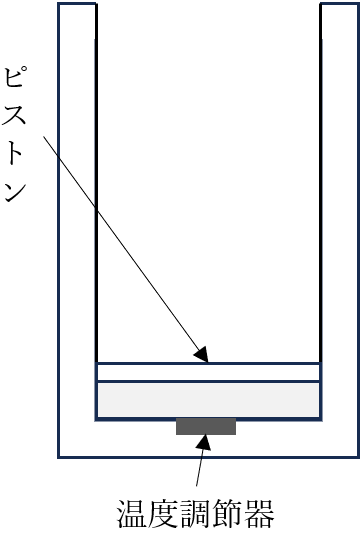
\includegraphics[width=12zw]{../graphs/jumon_61_1.png}
  \caption{}
\end{wrapfigure}
図1のように,断面積$S$〔$\text{m}^2$〕の細長い円筒型容器が鉛直に置かれている.
この容器内に,質量が無視できなめらかに動くことのできるピストンで,質量が$m\unit{g}$の水が隙間なく閉じ込められている.
容器内には温度調節器があり,容器内の物質を一様に加熱または冷却できるようになっている.
ピストンや容器は熱容量の無視できる断熱材でできており,外部との熱のやり取りはない.
次の問いに答えよ.

容器内の水を冷却して凍らせ,$-T_1\unit{℃}$で一定にした後,温度調節器の電力を一定にして,1気圧の大気圧のもとで加熱を続けた.
加熱し始めた時刻を0\,sとして,容器内の温度の変化を観測したところ図2のようになった.
すなわち,$t_1\unit{s}$後には0℃となりしばらく温度は一定となった.
加熱開始$t_2\unit{s}$後には氷は完全にとけて水になり,
その後再び温度が上昇し始め,加熱開始$t_\B\unit{s}$後には$T_\B\unit{℃}$に,
また$t_3\unit{s}$後には100℃となり,加熱開始$t_4\unit{s}$後には100℃の温度が保たれた.

\par}

\begin{enumerate}[(1)]
  \setlength{\leftskip}{-1.5zw}
  \setlength{\itemindent}{1zw}\setlength{\labelsep}{0.5zw}
  \setlength{\labelwidth}{1zw}\setlength{\leftmargin}{1zw}
  \setlength{\itemsep}{0.5\baselineskip}
  \item 水の比熱を$C_w$〔J/(g$\cdot$K)〕として,氷が完全にとけた直後の$m\unit{g}$の水が,0℃から$T_\B\unit{℃}$まで上昇する間に与えられた熱量を求めよ.
  \item 加熱している間の一定電力$P\unit{W}$を,$m,\,C_w,\,T_\B,\,t_\B,\,t_2$を用いて表せ.
  \item 氷の融解熱\unit{J/g}を,$C_w,\,T_\B,\,t_1,\,t_\B,\,t_2$を用いて表せ.
  \item 氷の比熱は,水の比熱の何倍か.$T_1,\,T_\B,\,t_1,\,t_\B,\,t_2$を用いて表せ.
  \item 加熱開始$t_\A\unit{s}$後に,この容器内に残っている氷の質量は,とけて水となっている部分の氷の質量の何倍か.$t_1,\,t_\A,\,t_2$を用いて表せ.ただし,$t_1<t_\A <t_2$である.
  \item 氷の蒸発熱\unit{J/g}と氷の融解熱の比を,$t_1,\,t_2,\,t_3,\,t_4$を用いて表せ.
\end{enumerate}

\begin{figure}[H]
  \centering
  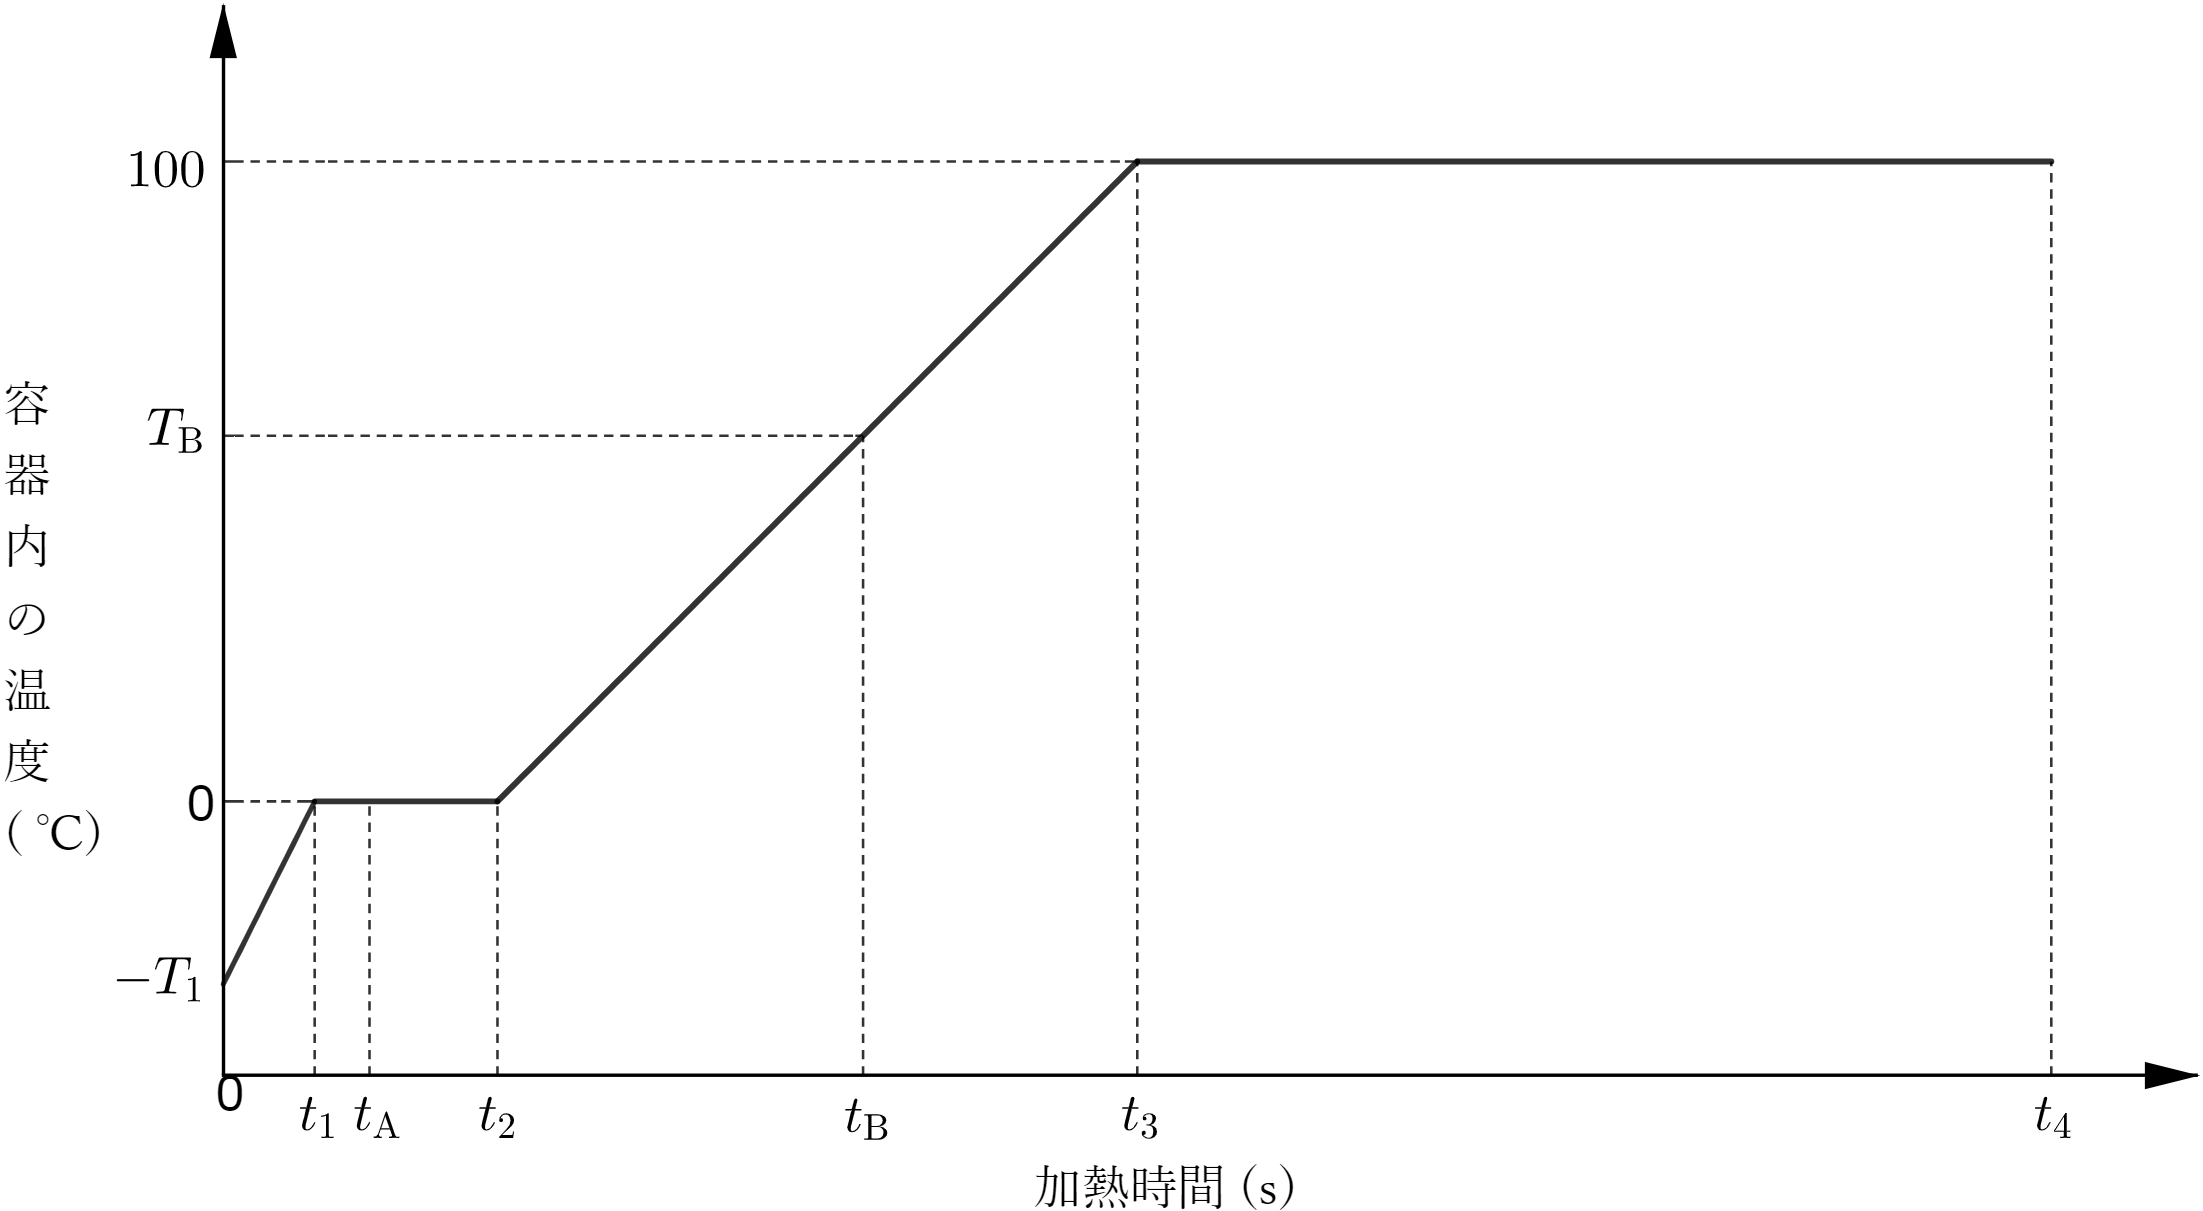
\includegraphics[width=.8\columnwidth]{../graphs/jumon_61_2.png}
  \caption{}
\end{figure}



% メモ
\begin{comment}

\end{comment}


%%%%%%%%%%%%%%%%%%
